\subsection{Administrationssystem}
Dette delsystem indeholder al funktionalitet til at manipulere produkter og produktkategorier. Dette indebærer oprettelse, sletning og redigering af produkterne og produktkategorierne. Administrationsystem er koblet op til CentralServer, og kommunikerer med denne via en Socket forbindelse (TCP/IP).

\subsubsection{Designovervejelser}
Designet af Administrationssystem startede ud med at lave en skitsering af, hvordan det grafiske skulle se ud. Dette betød at der skulle udvikles en grov skitse af designet\footnote{Skitse af designet kan ses i dokumentationen, side XYZ}.\\
Selve softwaren til Administrationssystem skulle sættes op på en måde, så det var overskueligt og modulært. I software design kurset blev der givet undervisning i designprincippet MVVM\footnote{Maybe something here?}, som forklarer, hvordan man kan dele sin GUI\footnote{Graphical User Interface} applikation op og adskille funktionalitet fra præsentation. Præsentation er det rent visuelle, altså opsætning af knapper, tekstbokse og så fremdeles. Funktionaliteten er den bagvedliggende hjerne i applikationen.\\
Administrationssystem softwaren var først lavet med funktionaliteten i codebehind\footnote{C\#-filen til XAML viewet}, hvilket hurtigt blev lidt rodet. Efter der i Softwaredesign forelæsningenblev det derfor besluttet af refactor koden så MVVM blev udnyttet.\\
Det visuelle design og funktionaliteten til at vise produkter og kategorier blev lavet i starten af udviklingen. Efter dette skulle kommunikationen mellem Administrationssystem og CentralServer på plads. Implementeringen af CentralServer satte en standard for, hvordan og hvornår data blev sendt frem og tilbage mellem CentralServer og de andre delsystemer, og derfor skulle der blot laves kommunikation for Administrationssystem der opfyldte disse krav. Det primære krav var, at Administrationssystem kontinuert skulle lytte på indkommende data, da der kunne blive sendt vigtig data på alle tidspunkter, også selvom den pågældende instans af Administrationssystem ikke havde anmodet CentralServer om noget.

\subsubsection{Implementering}
Det endelige design af Administrationssystemet er implementeret med MVVM som det primære design. Designet af den grafiske brugerflade holder sig op af det skitserede design.\\
Administrationssystem fungerer sådan, at ved start af programmet åbnes et hovedvindue, der viser systemets nuværende produkter samt produktaktegorier. Herfra er der knapper til resten af programmets funktionalitet, som indebærer opret, rediger og slet af produkter og kategorier. Produkter og kategorier kan markeres på den pågældende liste og ved sletning eller redigering slettes/ændres der på det markerede element.\\

Kommunikationen mellem Administrationssystem og CentralServer har to dele. Den første er at sende data til CentralServer, den anden er at modtage data. Den data der sendes og modtages er i XML-format. Et eksempel på data der bliver sendt og modtage mellem Administrationssystem og CentralServer kan ses på nedenstående sekvensdiagram, figur \ref{fig:adminsekvens}.

\begin{figure}[H]
	\centering
	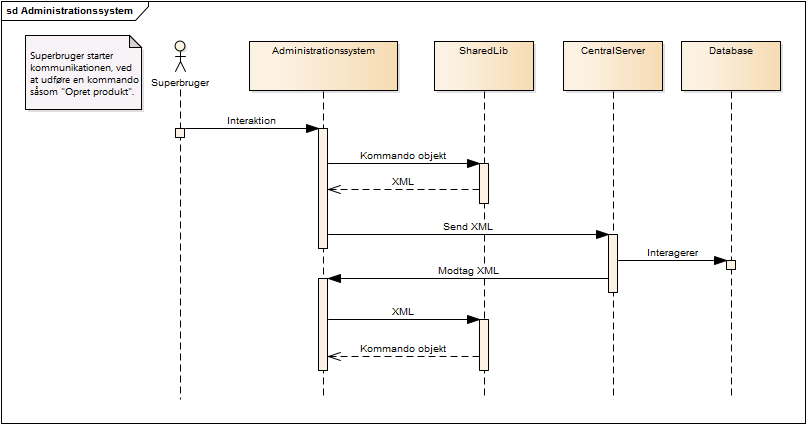
\includegraphics[width=0.8\textwidth]{Projektbeskrivelse/DesignOgImplementering/Images/Administrationssystem-sekvensdiagram}
	\caption{Kommunikation mellem Administrationssystem og CentralServer}
	\label{fig:adminsekvens}
\end{figure}